\chapter{Praxis}

Aktuell sind weltweit 28 Emissionshandelssysteme aktiv, die ca. 17\% der weltweiten Treibhausgasemissionen abdecken (vgl. \cite[S. 7]{icap.2023}).
Dieses Kapitel beschäftigt sich mit den Emissionshandelssystemen, die aktuell u.a. die deutsche Volkswirtschaft abdecken.
Stand Ende 2023 sind in Deutschland zwei Emissionshandelssysteme aktiv.
Zum einen das EU-Emissionshandelssystem (EU ETS), geregelt durch das 'EU ETS legislative framework' (vgl. \cite{eu.2023}), und zum anderen das deutsche nationale Emissionshandelssystem (nEHS), das durch das 'Brennstoffemissionshandelsgesetz' (BEHG) geregelt wird (vgl. \cite{dehst.2023}).
An diesen Emissionshandelssystemen werden Best Practices sowie auch Probleme und mögliche Lösungsansätze aufgezeigt.

\section{EU-Emissionshandelssystem (EU ETS)}

Das EU ETS ist das weltweit größte Emissionshandelssystem. Es wurde 2005 eingeführt und deckt ca. 40\% der Treibhausgasemissionen der EU ab. Es gilt für den europäischen Binnenmarkt sowie für die Staaten Island, Liechtenstein und Norwegen (vgl. \cite[S. 186]{hubert.2020}).
Es zielt auf direkte Emissionen aus der produzierenden Industrie, dem Energiesektor und der Luftfahrt ab. Ab 2024 sind auch Emissionen aus der Schifffahrt vom ETS abgedeckt (vgl. \cite{eu.2023}).
Bei dem EU ETS handelt es sich um einen sog. Downstream Emissionshandel (siehe Abb. \ref{fig:up_and_downstream_ets}) (vgl. \cite{dehst.2023}). 
Das bedeutet, dass Emittenten die Berechtigung für ihre eigenen Emissionen selbst erwerben. Ziel des EU ETS ist es, die Klimavorhaben der EU zu erreichen.
Das bedeutet mittelfristig die Treibhausgasemissionen bis 2030 im Vergleich zu 1990 um 55\% zu reduzieren und langfristig bis 2050 klimaneutral zu werden (vgl. \cite{eu.2023}). Schon jetzt wurden einige Erfolge erzielt. 
So konnten die Gesamtemissionen der von dem EU ETS abgedeckten Sektoren seit 2005 um 38\% reduziert werden (vgl. \cite{dehst3.2023}).
In der Energieindustrie ist der Ausstoß von $CO_2$e-Zertifikaten im Jahresschnitt von 2013 bis 2020 um 21\% gesunken (vgl. \cite{ub3.2023}).

Kern des EU ETS ist das für Emissionshandelssysteme klassische 'Cap and Trade' (vgl. \cite{eu.2023}). Genau wie in der Theorie werden die Zertifikate am Anfang via Auktionen ausgegeben und nachträglich an Zertifikatsbörsen wie dem European Energy Exchange (EEX) gehandelt (vgl. \cite[S. 186]{hubert.2020}) (vgl. \cite{eu.2024}).
Dennoch gibt es hier einige Besonderheiten. So erhalten Emittenten aus der Industrie einen Teil ihrer Berechtigungen von den Staaten kostenlos.
Grund dafür ist das sog. 'Carbon Leakage' (dt. Kohlenstoffleck) (vgl. \cite{eu2.2023}).
Dies beschreibt den Effekt, wenn Unternehmen treibhausgasintensive Produktionen ins Ausland verlagern, um so die Kosten des EU ETS zu umgehen und wettbewerbsfähig zu bleiben.
Um die Wettbewerbsfähigkeit der Industrie im europäischen Binnenmarkt zu sichern, werden deshalb bisher ein Teil der Berechtigungen kostenlos vergeben.
So kann sichergestellt werden, dass die Emissionen zumindest noch durch den 'cap' gedeckelt werden, auch wenn den Unternehmen die Kosten erspart bleiben.

Die kostenlose Ausgabe ist eine der größten Kritikpunkte am EU ETS. Um die Wettbewerbsfähigkeit der EU-Industrie trotzdem weiterhin zu sichern, wird nun mehr auf den 'Carbon Border Adjustment Mechanism' (CBAM) gesetzt (dt. Grenzausgleichsmechanismus) (vgl. \cite{ub.2023}).
Dieser wird schon seit Oktober 2023 angewandt und erhebt auf die Emissionen, die durch die Produktion von importierten Gütern nicht berücksichtigt wurden, eine Berichtigungsabgabe (vgl. \cite{ub2.2023}).
Diese soll bis 2026 den jeweiligen $CO_2$e-Preis der EU widerspiegeln (vgl. \cite{ub.2023}).
Im Gegensatz dazu wird die kostenlose Ausgabe von Zertifikaten für Branchen, die vom CBAM erfasst sind, zurückgefahren (vgl. \cite{ub.2023}).

Eine weitere Besonderheit des ETS ist die 'Market Stability Reserve' (MSR) (dt. Marktstabilitätsreserve) (vgl. \cite{eu3.2023}). Sie wurde Anfang 2019 eingeführt und soll auf der einen Seite den Zertifikatsüberschuss, resultierend aus der Finanzkrise, abbauen.
Damals wurde ein Überschuss an Zertifikaten von der EU in Umlauf gebracht, um die europäische Industrie zu entlasten.
Doch dieser Überschuss hat seit 2009 die Preise einbrechen lassen und so die Anreize für Unternehmen, ihre Emissionen zu reduzieren, geschwächt (vgl. \cite{eu3.2023}). Nach der Einführung der MSR ist der Preis innerhalb von wenigen Jahren stark angestiegen (siehe Abb. \ref{fig:price_co2_eu_ets}).
Auf der anderen Seite soll die MSR das EU ETS auch gegen externe Schocks absichern (vgl. \cite{eu3.2023}).
So werden jährlich abhängig von den 'Total Number of Allowances in Circulation' (TNAC) (dt. Anzahl der Zertifikate im Umlauf) entweder Zertifikate aus dem Markt in die MSR als Reserve überführt (TNAC über 833 Mio.) oder wieder ausgegeben (TNAC unter 400 Mio.) (vgl. \cite[S. 7]{icap2.2023}).
Um den o.g. Überschuss abzubauen, wurden von 2019 bis 2023 jährlich 24\% der Zertifikate, die im Umlauf waren, in die MSR überführt.
Danach soll die Einlagerung auf max. 12\% reduziert werden. Damit die MSR nicht so groß wird und es so zu einem Preiseinbruch kommen kann, kann sie maximal die Größe der ausgegeben Zertifikate aus dem Vorjahr haben.
Alle Zertifikate, die darüber hinaus in die MSR überführt werden sollten, werden gelöscht (vgl. \cite{eu3.2023}).
Im Rahmen des Klimapaketes 'Fit for 55' plant die EU-Kommission bis 2030, 24\% der Zertifikate im Umlauf in die MSR zu überführen und diesen nicht mehr auf die Größe des Vorjahres zu begrenzen, sondern fix auf maximal 400 Mio (vgl. \cite{ub.2023}).

\section{Nationales Emissionshandelssystem (nEHS)}

Seit 2021 hat Deutschland ein eigenes Emissionshandelssystem, das nationale Emissionshandelssystem (nEHS) (vgl. \cite{dehst.2023}). Es soll den EU ETS ergänzen, indem es auch die Emissionen aus den Sektoren Verkehr und Wärme abdeckt, die überwiegend von Privatpersonen erzeugt werden.
Damit nicht alle Privatpersonen direkt am nEHS teilnehmen müssen, wurde das nEHS als Upstream Emissionshandelssystem konzipiert (siehe \ref{fig:up_and_downstream_ets}) (vgl. \cite{dehst.2023}).
Das bedeutet, dass die Berechtigungen für die Emissionen von den Unternehmen erworben werden, die Brennstoffe, durch die später die Treibhausgasemissionen verursacht werden, in den Verkehr bringen (sog. BEHG-Verantwortliche).
Die Kosten werden dann an die Verbraucher weitergegeben, die dadurch einen Anreiz haben, emissionsärmere Technologien zu nutzen. Beispiel: Eine Raffinerie verkauft Benzin an eine Tankstelle.
Angenommen bei der Verbrennung von einem Liter Benzin entstehen 2,3 kg $CO_2$. Bei einem Preis von 45 €/t $CO_2$e entstehen so zusätzliche Kosten von 10,35 Cent pro Liter Benzin.
Die notwendigen Zertifikate dafür werden von dem BEHG-Verantwortlichen (Raffinerie) erworben und über den Händler (Tankstelle) an den Verbraucher weitergegeben.

Das 'Cap and Trade' wurde beim nEHS genau wie beim EU ETS von der Theorie abgewandelt (vgl. \cite{dehst.2023}).
In der Einführungsphase bis 2026 kann der Cap überschritten werden, da sich hier die Veräußerung von Zertifikaten nach der effektiven Nachfrage der BEHG-Verantwortlichen richtet.
Die EU-Klimaschutzverordnung verpflichtet Deutschland bei einer Überschreitung des Caps, dieses Defizit auszugleichen. 
Außerdem werden Emissionszertifikate bis 2025 nicht in einer Versteigerung, sondern zu einem Festpreis verkauft, der jährlich steigt (siehe Abb. \ref{fig:prices_nehs}) (vgl. \cite{dehst.2023}).
Ab 2025 werden die Zertifikate dann in einer Versteigerung ausgegeben.
Es bleibt aber dennoch ein Mindest- und Höchstpreis bestehen, in deren Rahmen sich dann auch der Preis je nach Nachfrage entwickeln wird.

Wie das EU ETS muss sich auch das nEHS des Problems des 'Carbon Leakage' stellen (vgl. \cite{dehst2.2023}). 
Anders als beim EU ETS gibt es hier auch Wettbewerbsnachteile im Vergleich zu anderen EU-Staaten, die sich ebenfalls im Binnenmarkt befinden.
So kann es z.B. zu Phänomenen wie dem 'Tanktourismus' kommen, bei dem Verbraucher, die in Grenzregionen leben, in andere EU-Staaten fahren, um dort günstiger zu tanken.
Während das EU ETS dieses Problem durch kostenlose Zertifikate für die Industrie und CBAM löst, bietet die Deutsche Emissionshandelsstelle (DEHSt) die Möglichkeit, sog. Beihilfen zu beantragen (vgl. \cite{dehst2.2023}).

Mittelfristig soll ab 2027 ein weiteres europaweites Emissionshandelssystem für diese Sektoren eingeführt werden (EU ETS 2) (vgl. \cite{ub.2023}).
Dieses soll genau wie das nEHS als Upstream Emissionshandelssystem konzipiert werden. Im Gegensatz zum nEHS sollen die Berechtigungen dirket versteigert und sich die Preise anschließend frei am Kohlenstoffmarkt bilden. 
Der nEHS wird dann in den EU ETS 2 überführt. So kann auch das Problem des EU-internen 'Carbon Leakage' gelöst werden.

\begin{figure}[ht]
	\centering
	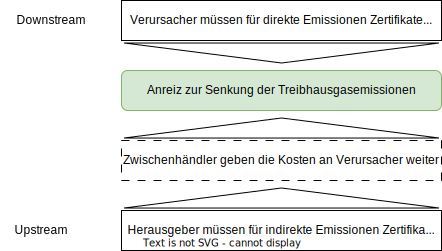
\includegraphics[width=0.8\textwidth]{Bilder/up_and_downstream_ets.png} 
	\caption{Anreize für Verursacher über Upstream- und Downstream-Systeme (vgl. \cite{dehst.2023})}
	\label{fig:up_and_downstream_ets}
\end{figure}

\begin{figure}[ht]
	\centering
	\includegraphics[width=1.0\textwidth]{Bilder/price_co2_eu_ets.png} 
	\caption{Preisentwicklung in € für Emissionsberechtigungen im EU ETS seit 2008 als $CO_2$e-Preis pro Tonne (\cite{dehst.2023})}
	\label{fig:price_co2_eu_ets}
\end{figure}

\begin{figure}[ht]
	\centering
	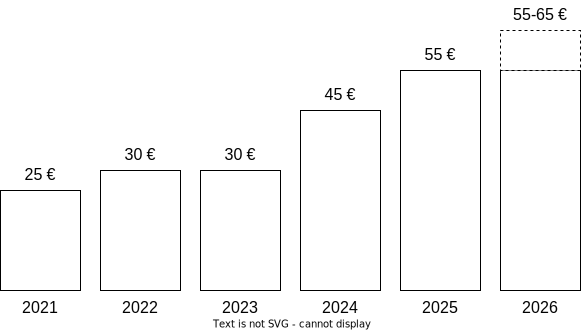
\includegraphics[width=1.0\textwidth]{Bilder/prices_nehs.png} 
	\caption{Preisentwicklung $CO_2$e-Preis pro Tonne für den nEHS (\cite{dehst.2023})}
	\label{fig:prices_nehs}
\end{figure}